\documentclass[a4paper,12pt]{article}

\usepackage{cmap}          % поиск в PDF
\usepackage{mathtext}         % русские буквы в формулах
\usepackage[T2A]{fontenc}      % кодировка
\usepackage[utf8]{inputenc}      % кодировка исходного текста
\usepackage[english,russian]{babel}  % локализация и переносы
\usepackage[left=2cm,right=2cm,top=2cm,bottom=2cm]{geometry}
\usepackage{amsfonts,amssymb,amsthm,mathtools} % AMS
\usepackage{amsmath}
\usepackage{icomma} % "Умная" запятая: $0,2$ --- число, $0, 2$
\usepackage{graphicx}
\usepackage{wrapfig} % картинка в тектсе
\usepackage{caption} % убирается номер у подписей caption*{}
\usepackage{csquotes} % цитаты
\usepackage{multirow} % для жестких таблиц
\usepackage{hhline}
\usepackage{indentfirst} % абзацный отступ после section
\usepackage{epigraph} % эпиграф
\usepackage{tikz}
\usepackage{pgfplots}
\usepackage[export]{adjustbox}
\usepackage{tabularx}
\usepackage{float}
\usepackage{longtable}

\title{\textbf{Измерение удельной теплоёмкости воздуха при постоянном давлении (2.1.1).}}
\author{Зайнуллин Амир Б05-206}

\begin{document}

\maketitle

\section{Аннотация}

\textbf{Цель работы:} 
измерить повышение температуры воздуха в зависимости от мощности
подводимого тепла и расхода при стационарном течении через трубу; исключив тепловые потери, по результатам измерений определить теплоёмкость воздуха при постоянном давлении.

\textbf{В работе используются:} 
Теплоизолированная стеклянная трубка; электронагреватель; источник питания постоянного тока; амперметр, вольтметр (цифровые мультиметры); термопара, подключенная к микровольтметру; компрессор; газовый счётчик;
секундомер.
	
\section{Теоретические сведения и методика измерений}

Теплоёмкость тела в некотором процессе определяется как их отношение: 
\begin{equation}
    C = \frac{\delta Q}{dT}
\end{equation}

\begin{figure}[H]
    \center{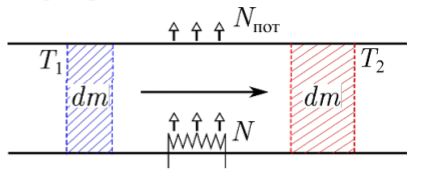
\includegraphics{lab_2_1_1}}
    \caption{Нагрев газа при течении по трубе}
\end{figure}

Рассмотрим газ, протекающий стационарно слева направо через трубу постоянного сечения, в которой установлен нагревательный элемент (см. рис. 1). Пусть за некоторое
время $dt$ через калориметр прошла
малая порция газа массой $dm=q dt$,
где $q$ [кг/с] — массовый расход газа в трубе. Если мощность нагрева равна $N$, мощность тепловых потерь на обмен с окружающей средой $N_{пот}$, то порция
получила тепло $\delta Q = (N-N_{пот})dt$. С другой стороны, по определению теплоёмкости (1): $\delta Q = c dm \Delta T$, где $\Delta T = T_{2}-T_{1}$ — приращение температуры	газа, и $c$ — удельная (на единицу массы) теплоёмкость газа в рассматриваемом процессе. При малых расходах газа и достаточно большом диаметре
трубы перепад давления на её концах мал, поэтому можно принять, что $P_{1} \approx P_{2} = P_{0}$, где $P_{0}$ — атмосферное давление. Следовательно, в условиях опыта
измеряется удельная теплоёмкость при постоянном давлении $c_{P}$. Таким образом, получаем
\begin{equation}
    c_{P} = \frac{N-N_{пот}}{q\Delta T}
\end{equation}
		 
\section{Эксперементальная установка:}
	
Схема установки изображена на рис. 2. Воздух, нагнетаемый компрессором, прокачивается через калориметр. Калориметр представляет собой стеклянную цилиндрическую трубку с двойными стенками, запаянными с торцов.
	
\begin{figure}[H]
	\begin{center}
    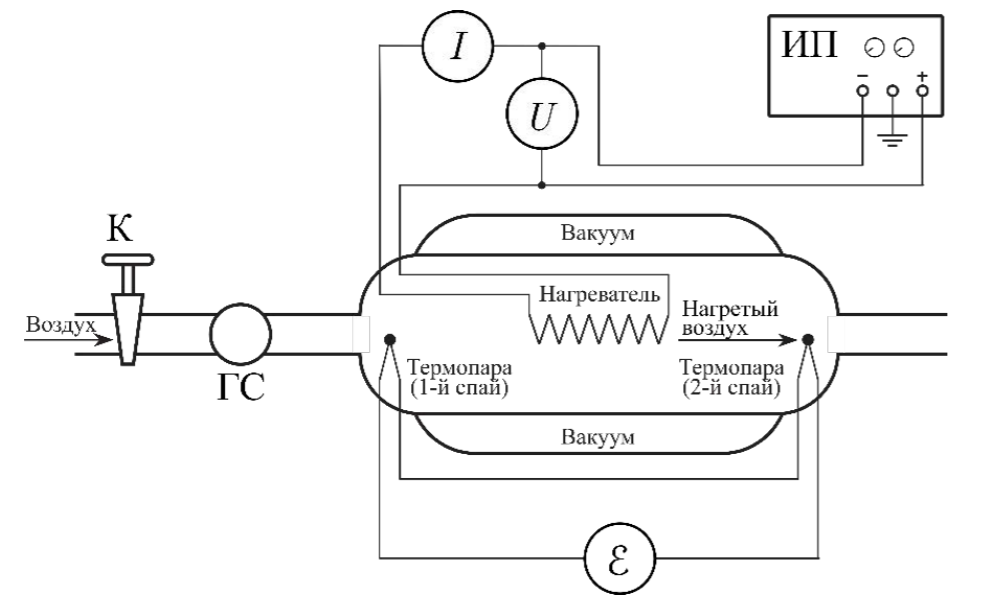
\includegraphics[width=0.8\textwidth]{lab_2_1_1_ust.png}
    \end{center}
    \caption{Схема эксперементальной установки}
\end{figure}
        
	
Мощность нагрева равна
\begin{equation}
    N= UI
\end{equation}

Для измерения разности температур $\Delta T$ служит медно-константановая термопара. Один спай термопары расположен в струе воздуха, входящего в
калориметр, и находится при комнатной температуре, а второй — в струе выходящего нагретого воздуха. Константановая проволока термопары расположена внутри калориметра, а медные проводники подключены к цифровому вольтметру. Возникающая в термопаре ЭДС $\varepsilon$ пропорциональна разности температур $\Delta T$ спаев: 
\begin{equation}
    \varepsilon =\beta \Delta T
\end{equation}

где $\beta = 40.7 \frac{мкВ}{^\circ C}$ — чувствительность медно-константановой термопары в рабочем диапазоне температур (20–30 $^\circ C$ ). ЭДС регистрируется с помощью микровольтметра.
		
Объём воздуха, прошедшего через калориметр, измеряется газовым счётчиком ГС. Для регулировки расхода служит кран К. Время $\Delta t$ прохождения
некоторого объема $\Delta V$ воздуха измеряется секундомером. Объёмный расход равен $\frac{\Delta V}{\Delta t} $, массовый расход может быть найден как 
\begin{equation}
    q = \rho_{0} \frac{\Delta V}{\Delta t}
\end{equation}
где $\rho_{0}$ — плотность воздуха при комнатной температуре, которая в свою очередь может быть получена из уравнения Менделеева–Клапейрона: $\rho_{0}= \frac{\mu P_{0} }{R T_{0}},$ где $P_{0}$ — атмосферное давление, $T_{0}$ — комнатная температура (в Кельвинах), $\mu = 29,0 {г/моль}$ — средняя молярная масса (сухого) воздуха.
		
Учитывая особенности устройства калориметра, следует ожидать, что мощность нагревателя расходуется не только на нагрев массы прокачиваемого воздуха, но и частично теряется за счет нагрева внутренних стенок термостата и рассеяния тепла через торцы термостата. Можно предположить, что при небольшом нагреве ($\Delta T \ll T_{0}$) мощность потерь тепла $N_{пот}$ прямо пропорциональна разности температур:

\begin{equation}
    N_{пот} = \alpha \Delta T
\end{equation}

где $\alpha$ — некоторая константа. При этом условии основное соотношение (2) принимает вид 

\begin{equation}
    N = (c_{P}q +\alpha)\Delta T
\end{equation}

Следовательно, при фиксированном расходе воздуха ($q = const$ ) подводимая мощность и разность температур связаны прямой пропорциональностью($\Delta T(N)$ — линейная функция).
		
\subsection*{Методика измерений}

\begin{enumerate}
    \item Подготовим к работе газовый счетчик.
    \item Охладим калориметр до комнатной температуры. 
    \item Проверим, что при постоянном расходе стрелка газового счетчика вращается равномерно.
    \item Запишем данные окружающей среды.
    \item Измерим несколько раз максимальный расход прокачиваемого воздуха. Найдем $q_{max}$. 
    \item Оценим величину тока нагревателя $I_0$, требуемого для нагрева воздуха на $\Delta T =$ 1 градус. Сравним с теоретическим значением.
    \item Проведем измерение зависимости разности температур от мощности
    нагрева $\Delta T(N)$ при максимальном расходе воздуха $q_1 = q_{\text{max}}$. Измерить 4-5 точек в диапазоне температур $\Delta T$ от ~2$^\circ C$ до ~10 $^\circ C$. После этого охладим калориметр до комнатной температуры.
\end{enumerate}

\section{Результаты измерений и обработка данных}
Данные окружающей среды

\begin{table}[H]
    \centering
    \begin{tabular}{|c|c|c|c|c|c|c|c|}
    \hline
        $P$, Па & $\sigma_P$, Па & $T$, К & $\sigma_T$, K & $\varphi$  & $P_н$, Па & $\rho_0$ кг/$м^3$ & $ \sigma_{\rho_0}$ кг/$м^3$ \\ \hline
        100300 & 100 & 295 & 0,1 & 0,48 & 2480 & 1,17 & 0,01 \\ \hline
    \end{tabular}
    \caption{Начальные условия}
\end{table}

Массовый расход найдем по формуле (5), найдя плотность по следующей формуле:
\[ \rho_0 = \frac{\mu \left(P_0 - \varphi P_{\text{н. п.}} \right)}{RT_\text{к}} = 1.17 \pm 0.01\ \frac{\text{кг}}{\text{м}^3}; \]


\subsection*{Измерения при первом расходе}
С помощью газового счетчика и секундомера измерим максимальный расход воздуха $\frac{\Delta V}{\Delta T}$ (в л/с). Измерения представлены в таблице 2. По найденным значениям определим среднее значение расхода и массовый расход воздуха $q_{max}$ [г/с].

\begin{table}[H]
    \centering
    \begin{tabular}{|c|c|c|c|c|c|c|}
    \hline
        № & $\Delta V$, л & $\sigma_V$, л & $\Delta T$, с & $\sigma_T$, с & $q_{max}$ г/с & $\sigma_q$ г/с \\ \hline
        1 & 5 & 0,05 & 52,14 & 0,3 & 0,112 & 0,003 \\ \hline
        2 & 5 & 0,05 & 52,12 & 0,3 & 0,112 & 0,003 \\ \hline
        3 & 5 & 0,05 & 52,3 & 0,3 & 0,112 & 0,003 \\ \hline
    \end{tabular}
    \caption{Измерение первого расхода}
\end{table}

\begin{table}[H]
    \centering
    \begin{tabular}{|c|c|c|}
    \hline
        $\langle q_{max} \rangle $ г/с & $\sigma_q^{случ}$ г/с & $\sigma_q^{сист}$ г/с \\ \hline
        0,112 & 0,0002 & 0,003 \\ \hline
    \end{tabular}
    \caption{Окончательные результаты}
\end{table}

Относительная погрешность косвенных измерений может быть найдена по формуле $$\frac{\sigma_{q_{max}}}{q_{max}} = \sqrt{(\frac{\sigma_{T_0}}{T_{0}})^2+(\frac{\sigma_{P_0}}{P_{0}})^2+ (\frac{\sigma_t}{t})^2}$$ 

% таблица 3
Окончательное значение расхода 
\[ q_{max} = 0.112 \pm 0.003 \; \frac{г}{с} \] 

Оценим величину тока нагревателя $I_{0}$, требуемого для нагрева воздуха на $\Delta T = 1$ К.
	
$C_p = 3.5R\mu \approx 1 \; \frac{Дж}{г\cdot K}.$
 	
Оценим минимальную мощность $N_0$, необходимую для нагрева газа при максимальном расходе. $N_{0} = c_{p}q\Delta T \approx 0.112 {Вт}.$
	
Учитывая, что сопротивление проволоки нагревателя составляет приблизительно $R_{н} \approx 35 \text{ Ом}$ и в процессе опыта практически не меняется, искомое значение тока $I_{0} = q N_{0} R_{н} \approx 56 \; {мА}.$
	
\bigskip
Проведем измерение зависимости разности температур от мощности нагрева $\Delta T(N)$ при максимальном расходе воздуха $q_0 = q_{max}.$
Следует отметить, что погрешность измерения тока: $\sigma_{I} = 0,4 \; мA$, а  напряжения: $\sigma_{U}= 0.03 \; мВ$.

\begin{table}[H]
    \centering
    \begin{tabular}{|c|c|c|c|c|c|c|c|c|}
    \hline
        $I, мA$ & $U, B$ & $N, Вт$ & $\sigma_N, Вт$ & $R_н$, Ом  & $\varepsilon, мВ$ & $\sigma_{\varepsilon}, мВ$ & $\Delta T$, K & $\sigma_{\Delta T}$, K \\ \hline111,3 & 3,831 & 0,426 & 0,003 & 34,42 & 0,124 & 0,006 & 3,05 & 0,15 \\ \hline
        138,8 & 4,782 & 0,664 & 0,003 & 34,45 & 0,189 & 0,009 & 4,64 & 0,23 \\ \hline
        183,5 & 6,333 & 1,162 & 0,004 & 34,51 & 0,335 & 0,017 & 8,23 & 0,41 \\ \hline
    \end{tabular}
    \caption{Результаты измерений при первом расходе}
\end{table}

По данным таблицы построим график.


\begin{figure}[H]
	\begin{center}
    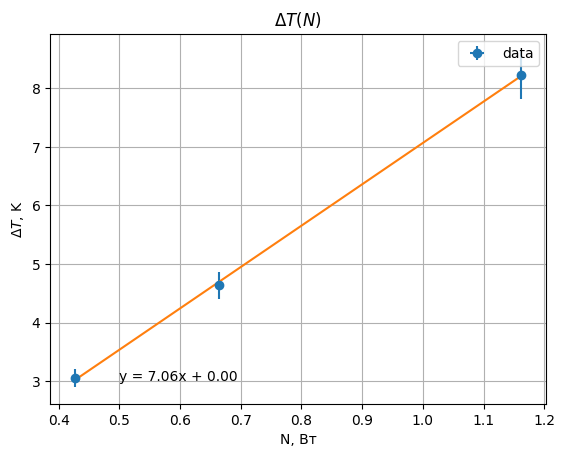
\includegraphics[width=0.8\textwidth]{first.png}
    \end{center}
    \caption{График для первого расхода}
\end{figure}

Найдем коэффициент наклона графика по МНК. 
\[ k_{1} = 7.06 \pm  0.13  \text{ К/Вт} \] 


\subsection*{Измерения при втором расходе}
Проведем те же измерения для второго расхода. 
\begin{table}[H]
    \centering
    \begin{tabular}{|c|c|c|c|c|c|c|}
    \hline
        № & $\Delta V$, л & $\sigma_V$, л & $\Delta T$, с & $\sigma_T$, с & $q_{max}$ г/с & $\sigma_q$ г/с \\ \hline
        1 & 5 & 0,05 & 30,74 & 0,3 & 0,191 & 0,005 \\ \hline
        2 & 5 & 0,05 & 30,75 & 0,3 & 0,191 & 0,005 \\ \hline
        3 & 5 & 0,05 & 30,66 & 0,3 & 0,191 & 0,005 \\ \hline
        4 & 5 & 0,05 & 30,64 & 0,3 & 0,191 & 0,005 \\ \hline
    \end{tabular}
    \caption{Измерение второго расхода}
\end{table}

\begin{table}[H]
    \centering
    \begin{tabular}{|c|c|c|}
    \hline
        $\langle q_{max} \rangle $ г/с & $\sigma_q^{случ}$ г/с & $\sigma_q^{сист}$ г/с \\ \hline
        0,191 & 0,0003 & 0,005 \\ \hline
    \end{tabular}
    \caption{Окончательные результаты}
\end{table}

Окончательное значение расхода 
\[ q_{max} = 0.191 \pm 0.005 \; \frac{г}{с} \] 

Полученная мощность и ток для этого расхода $N_{0} = c_{p}q\Delta T \approx 0.191$ Вт.

$I_{0} = \sqrt{\dfrac{N_0}{R_н}} \approx 73 \; {мА}.$
	

\begin{table}[H]
    \centering
    \begin{tabular}{|c|c|c|c|c|c|c|c|c|}
    \hline
        $I, мA$ & $U, B$ & $N, Вт$ & $\sigma_N, Вт$ & $R_н$, Ом  & $\varepsilon, мВ$ & $\sigma_{\varepsilon}, мВ$ & $\Delta T$, K & $\sigma_{\Delta T}$, K \\ \hline
        99,6 & 3,424 & 0,341 & 0,002 & 34,38 & 0,063 & 0,003 & 1,55 & 0,08 \\ \hline
        127,2 & 4,375 & 0,557 & 0,003 & 34,39 & 0,101 & 0,005 & 2,48 & 0,12 \\ \hline
        158,4 & 5,448 & 0,863 & 0,004 & 34,39 & 0,158 & 0,008 & 3,88 & 0,19 \\ \hline
        186,6 & 6,428 & 1,199 & 0,004 & 34,45 & 0,218 & 0,011 & 5,36 & 0,27 \\ \hline
        209,5 & 7,233 & 1,515 & 0,005 & 34,53 & 0,271 & 0,014 & 6,66 & 0,33 \\ \hline
        234,1 & 8,104 & 1,897 & 0,006 & 34,62 & 0,338 & 0,017 & 8,30 & 0,42 \\ \hline
    \end{tabular}
    \caption{Результаты измерений при втором расходе}
\end{table}

По данным таблицы построим график.

\begin{figure}[H]
	\begin{center}
    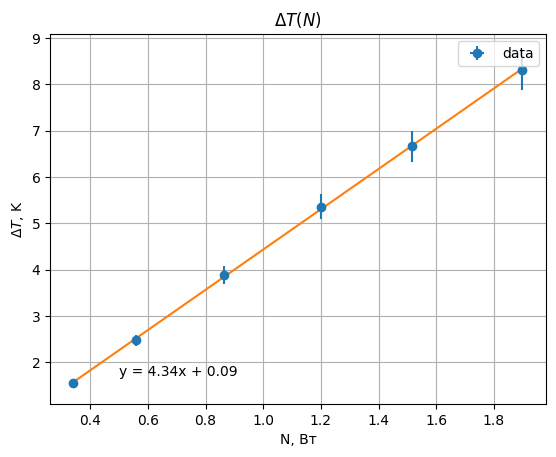
\includegraphics[width=0.8\textwidth]{second.png}
    \end{center}
    \caption{График для второго расхода}
\end{figure}

Найдем коэффициент наклона графика по МНК. 
\[ k_{2} = 4.34 \pm  0.03  \text{ К/Вт} \] 

\newpage

\subsection*{Зависимость наклона $k_{накл}$ от расхода $q$.}

Из уравнения (7) теоретических сведений найдем $\alpha$ и $c_P$, решив систему уравнений:
\[
	\left\{
		\begin{aligned}
			& c_P\, q_1 + \alpha = \frac{1}{k_1} \\
			& c_P\, q_2 + \alpha = \frac{1}{k_2}
		\end{aligned}
	\right.
\]
Путем математических преобразований получаем:
\[
\begin{aligned}
	 c_P = \frac{k_2 - k_1}{(q_1 - q_2)\, k_1\, k_2} & \qquad  \alpha = \dfrac{\dfrac{q_1}{k_2} - \dfrac{q_2}{k_1}}{q_1 - q_2} \\
	 c_P = 1124\ \frac{\text{Дж}}{\text{кг К}} & \qquad  \alpha = 0.016\ \frac{\text{Дж}}{K} 
\end{aligned}
\]
Оценим погрешности:

\[
	\sigma_{c_P} \approx c_P \sqrt{\left(\frac{\sigma_{k_1}}{k_1}\right)^2 + \left(\frac{\sigma_{k_2}}{k_2}\right)^2 + \left(\frac{\sigma_{q_1}}{q_1}\right)^2 + \left(\frac{\sigma_{q_2}}{q_2}\right)^2} = 47 \text{ } \frac{\text{Дж}}{\text{кг К}}
\]

\[ c_P  =   1124 \pm 47 \dfrac{\text{Дж}}{\text{кг К}} \] 
\[ \alpha = 0.016\pm 0.001\ \frac{\text{Дж}}{K} \] 

\section{Вывод}
\begin{enumerate}
    \item В данной лабораторной работе мы измеряли повышение температуры воздуха в зависимости от мощности подводимого тепла и расхода при стационарном течении через трубу. 
    \item По результатам измерений зависимости $\Delta T(N)$ построили графики для двух расходов. Нашли их коэффициенты наклона. Исходя из теоретической формулы (7) нашли теплоемкость воздуха при постоянным давлении.
    \item Сравним его с табличным. $c_{табл} = 1030 \frac{\text{Дж}}{\text{кг К}} $. Видно расхождение составило 8 процентов. Возможное расхождение могло получиться из за того, что теоретические упрощение, что мы измеряем при постоянном давлении не совсем так. Возможно в некоторых случаях мы не дожидались теплового равновесия при установлении новых условий. 
    \item Также видно, что график $\Delta T (N)$ для второго расхода не идет из нуля, возможно из за поспешного начала измерений.
    \item Мощность тепловых потерь в нашей лабораторной работе $N_{пот} = 0.016\pm 0.001\ \frac{\text{Дж}}{K}$
\end{enumerate}
\end{document}